\section{Grafos Computacionalmente}
A seguir iremos abordar alguns algoritmos de grafos, para facilitar o
entendimento em geral, será optado pelo uso de pseudo-linguagem nas
explicações, seguidos dos códigos em C++ e Python.

\subsection{Definição Computacional de Grafos}
Os grafos podem ser definidos computacionalmente de duas formas, veremos as
representações usando o grafo abaixo.
\begin{figure}[h]
	\centering
	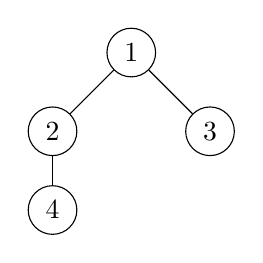
\begin{tikzpicture}[every node/.style={circle, draw, minimum size=0.6cm}]
		\node (1) at (0, 1) {1};
		\node (2) at (-1, 0) {2};
		\node (3) at (1, 0) {3};
		\node (4) at (-1, -1) {4};

		\draw (1) -- (2);
		\draw (1) -- (3);
		\draw (2) -- (4);
	\end{tikzpicture}
\end{figure}

\begin{itemize}
	\item \textbf{Lista de Adjacência: }A lista de adjacência é a maneira mais comum, ela funciona de uma maneira bem simples em cada posição $i$ da lista de adjacência haverá uma lista de vértices associados ao vértice $i$. Vejamos um exemplo:

	      \vspace{0.5cm}

	      %minipages criam blocos, esse está falando que vai usar 45% da largura disponivel para o texto, se quiser colocar tipo duas tabelas lado a lado, uso isso

	      %begin center cria um bloco que tudo vai ficar centralizado lá, ele já dá espaçamentos especiais

	      \begin{center}
		      \centering
		      $
			      \begin{array}{c|l} %cria um array (tabela), ela tem 2 colunas, basicamente está falando que a primeira coluna os dados ficam centralizados, tem uma | separando as colunas e a segunda os dados alinhasdos a esquerda
				      i & \text{Adjacências} \\ %aqui cria os rótulos das colunas o & separa
				      \hline %linha horizontal
				      1 & [2, 3]             \\ % cada \\ é pra pular uma linha
				      2 & [1, 4]             \\
				      3 & [1]                \\
				      4 & [2]                \\
			      \end{array}
		      $
	      \end{center}
	      \vspace{0.5cm}

	\item\textbf{Matriz de Adjacência: }é um pouco menos utilizada, mas basicamente as matrizes de adjacência tem uma ideia semelhante as listas de adjacência. Dado um grafo com $N$ vértices, você criará uma tabela (matriz) $N \times N$ em que cada linha representa um vértice $i$, e em cada coluna $j$, se o valor for diferente de 0, significa que há uma aresta de $i \rightarrow j$
	      \begin{center}
		      $
			      \begin{array}{c|cccc}
				      \text{Matriz} & \mathbf{1} & \mathbf{2} & \mathbf{3} & \mathbf{4} \\
				      \hline
				      \mathbf{1}    & 0          & 1          & 1          & 0          \\
				      \mathbf{2}    & 1          & 0          & 0          & 1          \\
				      \mathbf{3}    & 1          & 0          & 0          & 0          \\
				      \mathbf{4}    & 0          & 1          & 0          & 0          \\
			      \end{array}
		      $
	      \end{center}

	      Podemos trocar e usar valores diferentes de 1 e representar grafos ponderados,

\end{itemize}

